\documentclass{anstrans}
%%%%%%%%%%%%%%%%%%%%%%%%%%%%%%%%%%%
\title{}
\author{Baptiste Mouginot,$^{*}$ Kathryn Mummah,$^{*}$ Paul P.H.  Wilson$^{*}$}

\institute{
$^{*}$University of Wisconsin-Madison, WI
}

\email{mouginot@wisc.edu \and mummah@wisc.edu \and paul.wilson@wisc.edu}

% Optional disclaimer: remove this command to hide
% \disclaimer{Notice: this manuscript is a work of fiction.  Any resemblance to
% actual articles, living or dead, is purely coincidental.}

%%%% packages and definitions (optional)
\usepackage{graphicx} % allows inclusion of graphics
\usepackage{booktabs} % nice rules (thick lines) for tables
\usepackage{microtype} % improves typography for PDF
\usepackage{float}

\newcommand{\SN}{S$_N$}
\renewcommand{\vec}[1]{\bm{#1}} %vector is bold italic
\newcommand{\vd}{\bm{\cdot}} % slightly bold vector dot
\newcommand{\grad}{\vec{\nabla}} % gradient
\newcommand{\ud}{\mathop{}\!\mathrm{d}} % upright derivative symbol


\usepackage[acronym]{glossaries}
\newacronym{UOX}{UOX}{uranium oxide fuel}
\newacronym{MOX}{MOX}{mixed oxide fuel}
\newacronym{LWR}{LWR}{light water reactor}
\newacronym{SFR}{SFR}{fast breeder reactor}

\begin{document}
%%%%%%%%%%%%%%%%%%%%%%%%%%%%%%%%%%%%%%%%%%%%%%%%%%%%%%%%%%%%%%%%%%%%%%%%%%%%%%%%
\section{Introduction}

Fuel cycle simulations, as with any simulation process, do not produce results
without uncertainties.  Those uncertainties have different sources: data uncertainties (from
the simulator's reliance on previously estimated/measured data), modeling
uncertainties (from simplifications made by the simulator). This work we will be
focused a part of the data uncertainty related to the expected behavior of the
facilities being simulated.

Simulation errors could be important in the context of treaty verification.
Some scenarios require estimating historical fissile material production based
on records of facility operation and material transfer.  If the measurements of
facility operation and material transfer are subject to uncertainty, the total
production quantities will then also be uncertain.  Any uncertainty in fissile
production quantities poses a material accounting challenge, possibly creating
an opportunity for undetected diversion.  

This study seeks to understand which measures of facility operation have the
most impact on the uncertainty of fissile material production across a complete
fuel cycle.  Uncertainty propagation using a Monte Carlo method will be applied
to the Cyclus fuel cycle simulator \cite{cyclus} to estimate the effect of
individual facility uncertainties on the output metrics. The same simulation
will be simulated $N$ times, for each simulation parameters affected with an
uncertainty will be randomly determined, the distribution of each output metrics
over the N iterations of the simulation, will be used to estimate their
respective uncertainty.

\section{The Experiment}

\subsection{Method}

To estimate the uncertainty of fuel cycle output metrics, a Total Monte
Carlo approach has been applied.  In each of 199 independent simulations,
some of the parameters that define facility behavior are randomly selected
from Normal distributions with standard deviations that are $10\%$ of the mean
value.  This artificially large standard deviation is selected for the purpose
of demonstrating the methodology.  The mean and standard deviation of some
output metrics are calculated from the simulation output, as a function of time.

To pursue this work, both the Cycamore\footnote{Low
fidelity facilities package for Cyclus}\cite{cycamore} and the
CyCLASS\footnote{Reactor and fuel fabrication facility based on CLASS\cite{CLASS} models}\cite{mouginot_2018, cyclass} packages were
updated to evaluate the uncertainty of several
operational parameters in their associated facilities.  Table
\ref{tab:package_uncertainty} summarizes all uncertainty-tracking modifications implemented in the
facilities of Cycamore and CyCLASS.

\begin{table}[htb]
\centering
  \caption{Summary of facility modifications according to their Cyclus archetype package.}
\begin{tabular}{cl|l}
\toprule

Package   & Facility   & Parameters                \\
\midrule
Cycamore & Separation & Separation efficiency     \\\cmidrule{2-3} 
         & Storage    & Residence Time            \\
\midrule
CyCLASS  & Reactor    & Cycle Length              \\
         &            & Power                     \\
         &            & Fuel Enrichment (PWR-UOX) \\

\bottomrule
\end{tabular}

  \label{tab:package_uncertainty}
\end{table}

The uncertainty of the different parameters in this study
are systematic for each new deployed facility: each time a new facility is
deployed (such as a reactor or a fuel fabrication facility) a new set of
parameters are sampled, and those parameters are used throughout the life
of that facility.

\subsection{The Fuel Cycle Scenario}
For demonstration purposes, a simple commercial fuel cycle transition is used,
inspired from the EG23 fuel cycle
of the Nuclear Fuel Cycle Evaluation and Screening Report\cite{ES}.
Pictured in Figure \ref{fig:cycle}, this is a
transition from a \gls{LWR} fleet loaded with \gls{UOX} fuel to a
\gls{SFR} fleet loaded \gls{MOX} fuel, considering a $1\%/$y growth
of the nuclear generated power (Figure \ref{fig:power}).
\begin{figure}[ht] % replace 't' with 'b' to force it to be on the bottom
  \centering
  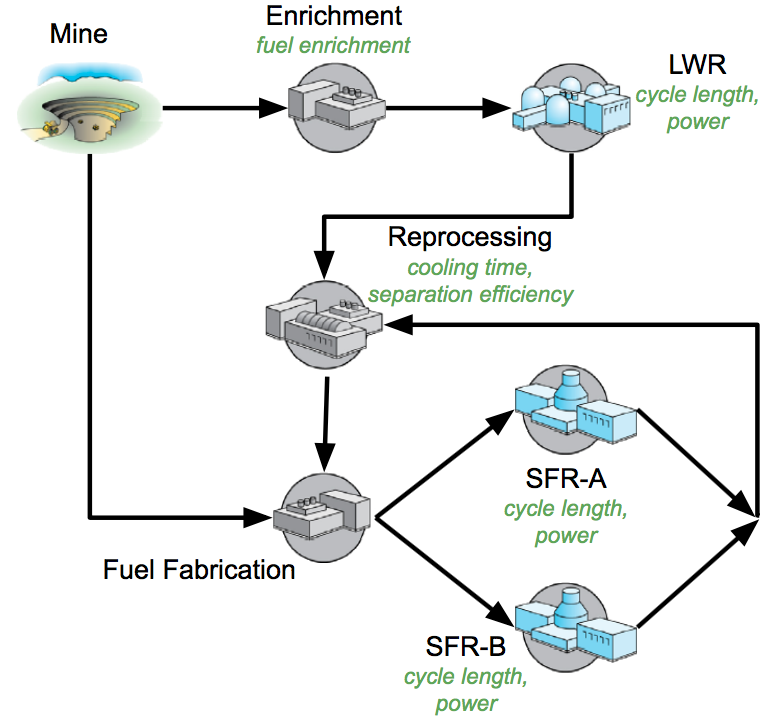
\includegraphics[scale=0.31]{cycle.png}
  \caption{Simplified representation of the material flow between the different facilities,
  with each operational parameter associated with an
  uncertainty labeled in green.}\label{fig:cycle}
\end{figure}


As illustrated in Figure \ref{fig:power}, the transition starts with a fleet
composed of only \glspl{LWR} loaded with enriched \gls{UOX} fuel.  The actual
transition starts around year 35, with the deployment of \glspl{SFR}. The \glspl{SFR} are loaded
with \gls{MOX}, which consists of plutonium blended with natural
uranium.

\begin{figure}[ht] % replace 't' with 'b' to force it to be on the bottom
    \centering
    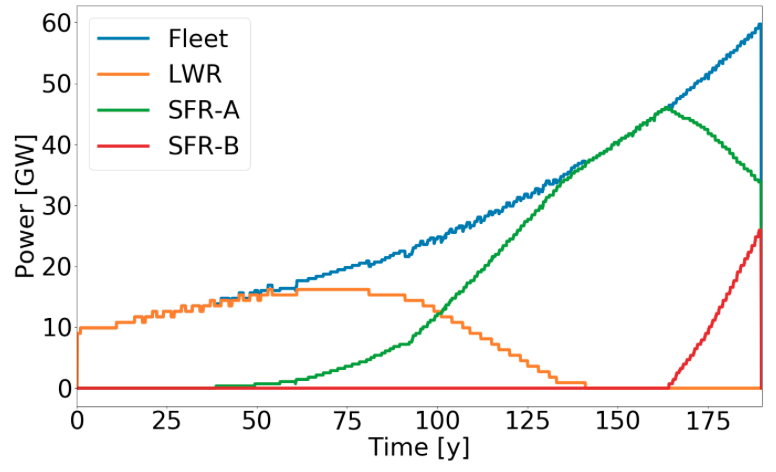
\includegraphics[scale=0.18]{power.png}
    \caption{Electric power generated over time, with the full production,
        the \gls{LWR} contribution, and the \gls{SFR} contribution labeled in blue, orange, and green, respectively.}
    \label{fig:power}
\end{figure}


The plutonium, required for \gls{MOX} fabrication, is reprocessed from all
used fuel.  At first, it is sourced only from \gls{UOX}, then used \gls{MOX} fuel
as it becomes available for reprocessing.

Both fuel reprocessing and fabrication rate are both limited by the facilities
throughput and the ressource available.  The enrichment of the \gls{UOX} is processed
on demand.  Buffer storage facilities (not shown in Figure \ref{fig:cycle}) are present
between all facilities with constant processing rates.

In this work, a time step of 1 month has been considered, i.e., each output
metric is reported once per month. Additionally, decay processes have not be
taken into account.  

It must be noted that for this work, the fuel enrichment was determined by a
fuel fabrication model\cite{Leniau2015125} which
calculates the fissile fraction required in the fuel to reach a given target
burnup at the end of irradiation.  Therefore, the uncertainty of the fuel
enrichment is not applied directly to the effective enrichment. It is instead applied to the
burnup, which appears to lead to a fuel enrichment uncertainty close to
$10\%$.

For each of the parameters in Table \ref{tab:package_uncertainty}, a set of
199 simulations was performed with only that parameter being randomly varied.
An additional set of 199 simulations was performed in which all five
parameters are randomly varied.  A reference simulation was performed
with all five parameters fixed at the mean value.



\section{Results}

Because the main interests of nuclear archaeology involve highly enriched uranium production and
fissile inventories, this study mainly focuses on the uncertainties of
the total quantity of natural uranium used and the total unused fissile
inventory (separated plutonium).
Generated power is also briefly investigated to ensure the overall
uncertainty is not contaminated with a missed fuel loading, which could
be interesting but is not the focus of this work. It is assumed that no reactor
are unexpectedly shutdown because of fuel shortage, as such events should be well
documented...

At each time step, the $\pm1\sigma$ uncertainty due to the full set of varied
parameters is reported.  In addition, the relative contribution to the total
uncertainty from each of the parameters is calculated as the ratio of the
$1\sigma$ uncertainty due to that parameter over the total uncertainty.

\subsection{Generated Power}

\begin{figure}[t] % replace 't' with 'b' to force it to be on the bottom
    \centering
    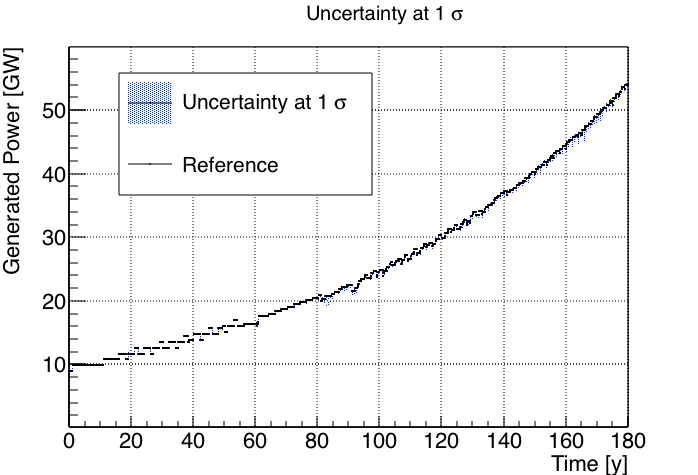
\includegraphics[scale=0.36]{power_full}
    \caption{Electric power generated as a function of time.  The black line
        represents the reference calculation and the blue zone
        represents the 1 $\sigma$ uncertainty distribution.}\label{fig:power_full}
\end{figure}

By design, the very low uncertainty (Figure \ref{fig:power_full}) on the
generated power is expected.
Indeed the transition scenario has been designed to allow all the reactors to
receive the fuel as needed allowing them to be producing power all the time.
This ensures that the measured uncertainty is not affected by a facility
disruption that has an outsized impact on material flows.
As \gls{SFR} fuel is built from
reprocessed used fuel, the availability of that used fuel may impact the
capability to build the required MOX-SFR fuel.  Facility disruptions may
cause material shortages that can lead to snow-ball effect of more disruptions
later in the simulation.  While such disruptions are interesting in some analyses,
they are outside the scope of this study.

\subsection{Natural Uranium Consumption dedicated to PWR-UOX fabrication}

Figure \ref{fig:unat_full} represents the cumulative natural uranium consumption
dedicated to PWR-UOX fuel fabrication as a function of time.  The uncertainty on
the cumulative uranium consumption grows as expected with the time and the
loading of the \glspl{LWR}.  The increase stops around year 125y with the
decommissioning of the last \glspl{LWR}.

\begin{figure}[ht] % replace 't' with 'b' to force it to be on the bottom
    \centering
    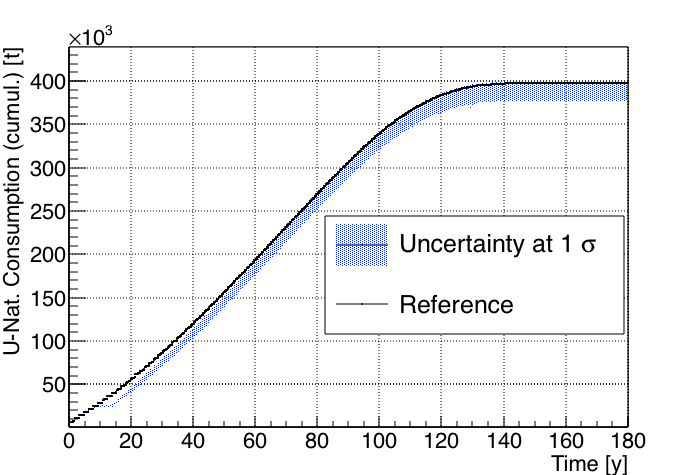
\includegraphics[scale=0.35]{unat_full}
    \caption{Cumulative consumption of natural uranium as a function of time.  The black line
        represents the reference calculation and the blue zone
        represents the 1 $\sigma$ uncertainty distribution.}\label{fig:unat_full}
\end{figure}


As expected, cooling time, separation efficiency and thermal power do not
affect the natural uranium consumption.  The uncertainty on the natural uranium
consumption is dominated by the \gls{LWR} cycle length: shorter the cycle
length is, the more fuel will be loaded.


\begin{figure}[h!!] % replace 't' with 'b' to force it to be on the bottom
    \centering
    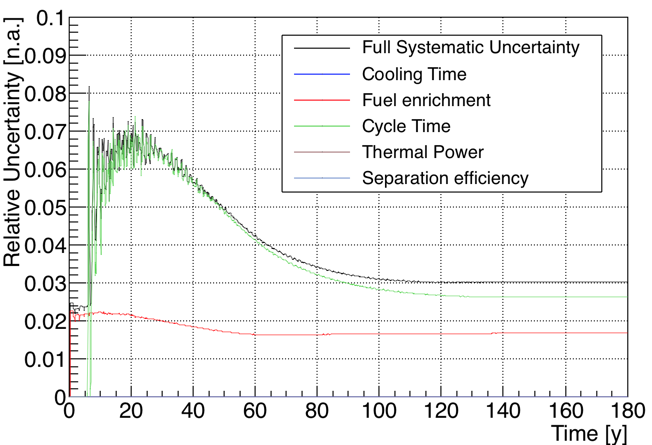
\includegraphics[scale=0.35]{unat_uncer}
    \caption{Cumulative natural uranium consumption relative uncertainty, with
    in black the total uncertainty at 1$\sigma$, and in color the uncertainty
    contribution of each parameter: cooling time (blue), fuel enrichment (red),
    cycle time (green), thermal power(brown), separation efficiency (light
    blue).}\label{fig:unatr_uncer}
\end{figure}
The relative uncertainty of the total uranium consumption starts at about
$5.5\%$ a slowly drops and stabilise around $3\%$.

Uncertainty fluctuation of the full relative uncertainty can be observed before
year 50.  Those fluctuation are induced by the fuel loading: all reactors at the
beginning of the simulation have synchronised cycle, this phenomenon disappears
with the gradual decommissioning of the initial reactors, spread on 50 years.

The decrease of the cycle time uncertainty contribution, from year 30 to year
90, can be understood as an averaging effect.  As the uncertainty are defined once
per deployed facility, each reactor will have a different cycle
length value, so a different number of batches loaded per year.  With the increase
of deployed reactors, the number of batches of \gls{LWR} fuel loaded converges
to the references one, reducing its impact on the uncertainty on the total
uranium consumption. This uncertainty contribution to the overall uncertainty
decrease is proportional to the number of \gls{LWR} reactors and stops with the
decommission of the last one.

The fuel enrichment contribution follow a close to constant uncertainty
contribution of $2\%$, so as the total relative uncertainty decrease, it
has a growing shared of the total uncertainty over time.

\subsection{Fissile Inventory}
The fissile inventory corresponds to the amount of separated fissile material waiting to
be blended with natural uranium in order to produce the \gls{SFR} MOX fuel.

As observed on Figure \ref{fig:pu_full}, the fissile inventory starts to grow in
year 40, with the deployment of the first reprocessing facility.  It grows
during the first period of the \glspl{LWR} to \gls{SFR}-A transition until
year 90, then decrease slightly as the last \glspl{LWR} are decommissioned.
When he steady state is reached (full \gls{SFR} fleet), the plutonium
inventory starts to increase, as the breading ratio of the \glspl{SFR} is higher
than the deployment needs.

\begin{figure}[ht] % replace 't' with 'b' to force it to be on the bottom
    \centering
    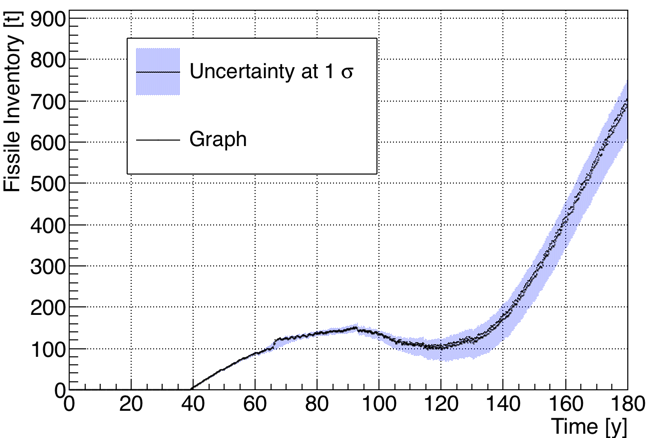
\includegraphics[scale=0.35]{pu_full}
    \caption{Fissile (plutonium) inventory as a function of time.  The black line
        represents the reference calculation and the blue zone
        represents the 1 $\sigma$ uncertainty distribution.}\label{fig:pu_full}
\end{figure}

\begin{figure}[h!!] % replace 't' with 'b' to force it to be on the bottom
    \centering
    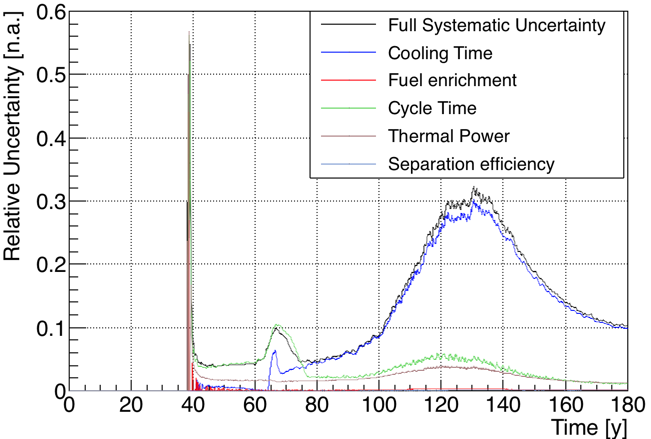
\includegraphics[scale=0.35]{pu_uncer}
    \caption{Fissile (plutonium) inventory relative uncertainty, with
    in black the total uncertainty at 1$\sigma$, and in color the uncertainty
    contribution of each parameter: cooling time (blue), fuel enrichment (red),
    cycle time (green), thermal power(brown), separation efficiency (light
    blue).}\label{fig:pu_uncer}
\end{figure}

Regarding the uncertainty, disregarding the artefact of a very low mean inventory
observed at the onset of fissile material production, the relative uncertainty
starts at about $5\%$, and grows until year
125 to decrease to $10\%$ at the end of the simulation time (180y), it seems
it would have reached an equilibrium between $5$ and $10\%$ with longer
simulations...
Between year 40 and 70, the main contributor to the fissile inventory
uncertainty is the cycle length.  As with the uranium needs, different cycle length
implies different number of fuel loads, so different amount of resources used.  Never the less, around year 65 (see Figure
\ref{fig:used_fuel}), the stock of used fuel available for reprocessing becomes
small enough to start limiting the production of fissile material.
The uncertainty weight is then slowly transferred from
the cycle length to the fuel cooling time.

\begin{figure}[ht] % replace 't' with 'b' to force it to be on the bottom
    \centering
    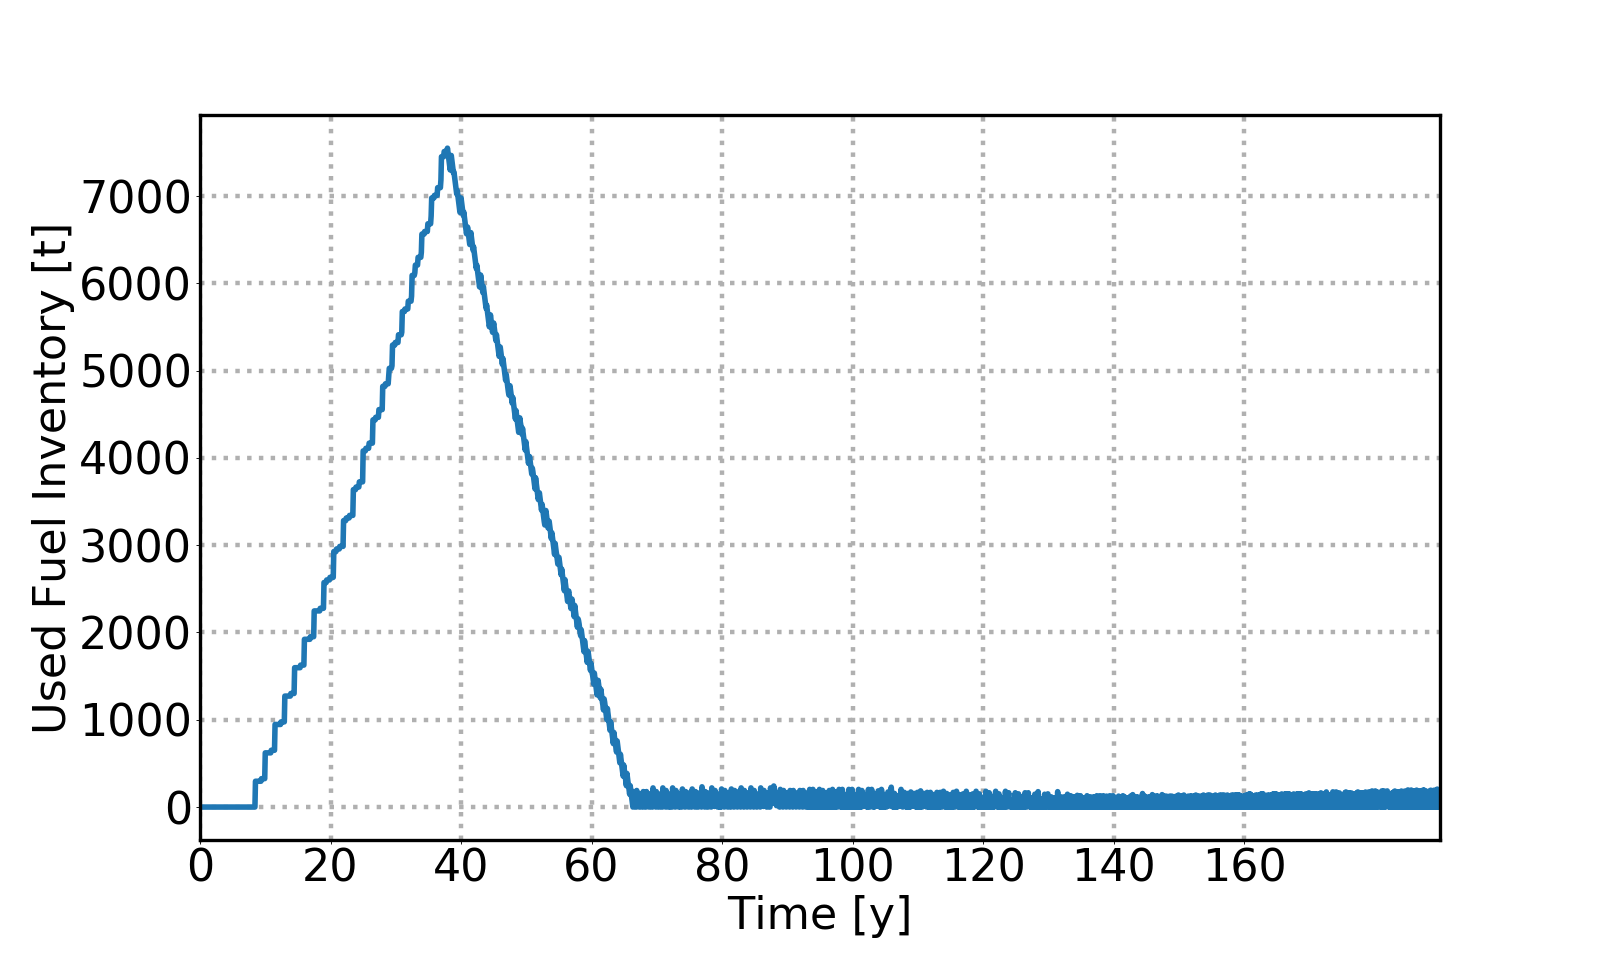
\includegraphics[scale=0.18]{used_fuel}
    \caption{Used fuel inventory, corresponding to the amount of used
    \glspl{LWR} and \glspl{SFR} fuel, cooled and waiting to be reprocessed.}
    \label{fig:used_fuel}
\end{figure}
Between year 90 and 120, the \gls{SFR} deployment speed increases, it has to
compensate the non replacement of the decommissioned \glspl{LWR} as well as
follow the power demand.  During this period the needs in plutonium are higher
than its productions, explaining the observed decrease of the total amount, and
the increase associated relative uncertainty.

As the transition ends, the plutonium breed from the \glspl{SFR} starts to be
sufficient to sustain the new \glspl{SFR} deployment to follow the power demand.

It is also interesting to note that, the uncertainty contribution from the cycle
length is between year 40 and 70 comes mainly from fuel batch loading
frequencies, and after it relative contributions follows closely the thermal
power one, suggesting a contributions through fuel discharge burnup (i.e.  fuel
discharge composition).

\subsection{Discussion}

Uranium consumption and separated fissile inventory are two important metrics
regarding to non proliferation and nuclear archaeology.  In this study, we have
been able to estimate than the cycle length uncertainty of $10\%$ implies a
variation of $3\%$ to $5\%$ on the total uranium needs uncertainty, where about
$10\%$ on the enrichment implies a almost flat uncertainty of $2\%$.

Regarding the reprocessed fissile inventory, this study has shown the limited
impact of the reprocessed fuel compositions (through burnup variations) it
limited to $5\%$, where fuel availability constrains, fuel loading frequency (cycle
time), or fissile materials available for fuel fabrication (cooling time) can lead to higher
uncertainties, respectively up to $10\%$ and to $30\%$.  Moreover it is very
interesting to observe the pressure transition from one to the other around
year 70.

This preliminary study may suggest that the most important contribution to
natural uranium consumption and fissile inventory is coming from the time when
occurs the different material exchange between facilities, and not necessary
from the physical parameters such as thermal power or fuel enrichment. Further
analysis should allow us to confirm or denies it.

\section{Conclusion}

Two main points can be deduced from this work.  Firstly, in a transitional
fuel cycle, the uncertainty contributions to an output metric can vary over time
depending of various factors: deployment schedule artifact or pressure point in
the material flows.

Secondly, it is important to note the special character of the time related
parameters uncertainty in a fuel cycle study, such as cooling time and cycle
length.  Where some of those time related parameter will on the first order only
impact material availability (as the cooling time will do), some other, like
cycle length, will also have a impact as physical parameters such as fuel
enrichment or thermal power.  

Cycle length impacts the discharge fuel burnup, it also affects the frequency of
the fuel loads, this, as well as the cooling may imply a uncertainty on the
material availability, which could lead to an artificially large uncertainty.
Those kind of time related uncertainties will require a careful analysis on further
uncertainty analysis, in order to understand and measure accurately their
contributions on uncertainties.

This study aims to be a proof-of-principle for uncertainty propagation in
potential commercial fuel cycle transition.  While it has demonstrated the
capability to measure the uncertainty on output fuel cycle metrics and their
relative contributions, it has only been applied to systematic uncertainties per
facilities (parameters randomly generated at each new facility deployment).
This kind of study will to be extended to random uncertainty (new parameter
values at each occurrence) and completely systematic uncertainty (shared by all
the facilities of a kind).

While the parameters contributing to natural uranium needs and fissile inventory
uncertainties might be obvious, such study allows to estimate each parameters
contribution, it could be less obvious for other parameters, such as
plutonium quality, waste compositions.  Such studies could also provide research
guidance for nuclear archaeology works, which aims to precisely estimate past
fissile production by the different nuclear countries.



%%%%%%%%%%%%%%%%%%%%%%%%%%%%%%%%%%%%%%%%%%%%%%%%%%%%%%%%%%%%%%%%%%%%%%%%%%%%%%%%
%% \appendix
%% \section{Appendix}
%%
%% Numbering in the appendix is different:
%% \begin{equation} \label{eq:appendix}
%%   2 + 2 = 5\,.
%% \end{equation}
%% and another equation:
%% \begin{equation} \label{eq:appendix2}
%%   a + b = c\,.
%% \end{equation}
%%
%%%%%%%%%%%%%%%%%%%%%%%%%%%%%%%%%%%%%%%%%%%%%%%%%%%%%%%%%%%%%%%%%%%%%%%%%%%%%%%%
%% \section{Nomenclature}
%%
%% \begin{table}[H]
%%     \centering
%%     \begin{tabular}{l|l}
%% %         &  \\
%%         $N$ & Feed assay \\
%%         $N'$ & Product assay \\
%%         $N''$ & Tails assay \\
%%         $\alpha$ & Feed to product enrichment factor \\
%%         $\beta$ & Feed to tail enrichment factor \\
%%         $\theta$ & Cut
%%     \end{tabular}
%% %    \caption{Caption}
%%     \label{tab:my_label}
%% \end{table}

%% \begin{figure}[ht] % replace 't' with 'b' to force it to be on the bottom
%%   \centering
%%   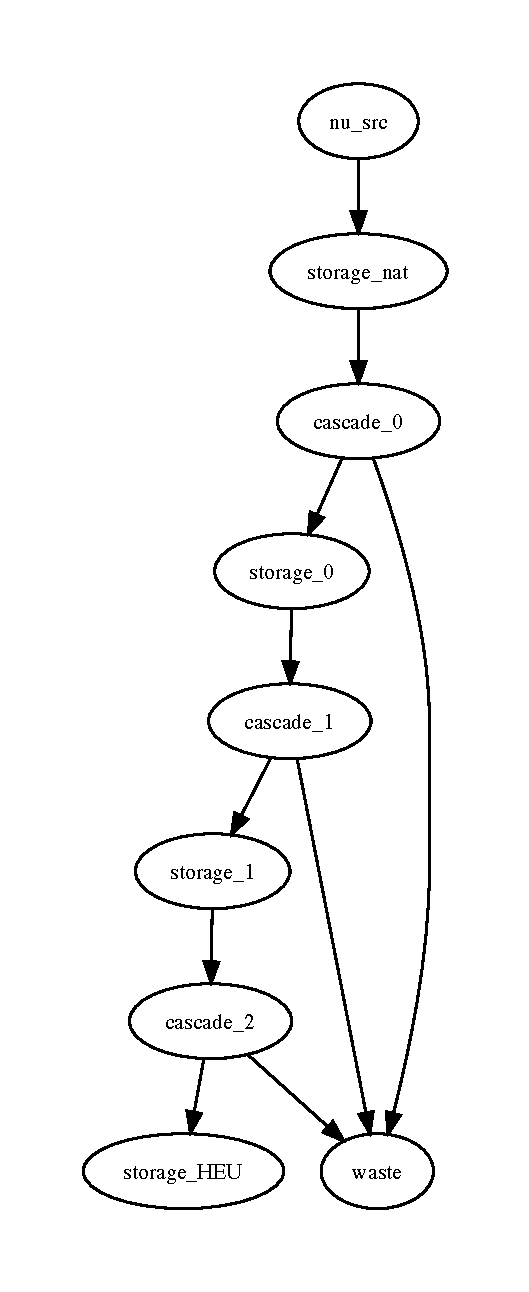
\includegraphics[scale=0.68]{flow_case_2_no_recy.pdf}
%%   \caption{Illustration of the material flow between the different level of
%%       cascades without tail recycling, in this diagram, nu\_src corresponds to
%%       an infinite source of natural uranium, cascade\_ $\{n\}$ and storage\_
%%       $\{n\}$ to the cascade and the storage getting the products of the
%%       cascades at the level $\{n\}$.}\label{fig:flow}
%% \end{figure}

%% \begin{table}[htb]
%% \centering
%%   \caption{Summary of cascade properties for each level.}
%% \begin{tabular}{cllll}
%% \toprule
%%
%% Level   &           & Assay     &       & Machines  \\
%%         & Feed      & Product   & Feed  &           \\
%% \midrule
%% 0       & 0.0071    & 0.0413    & 0.0029 & 167       \\
%% 1       & 0.0413    & 0.2043    & 0.0173 & 169       \\
%% 2       & 0.2043    & 0.5941    & 0.0971 & 168       \\
%% 3       & 0.5941    & 0.8834    & 0.3915 & 168       \\
%% 4       & 0.8834    & 0.9735    & 0.7746 & 169       \\
%%
%% \bottomrule
%% \end{tabular}
%%
%%   \label{tab:cascadelvl}
%% \end{table}

%%%%%%%%%%%%%%%%%%%%%%%%%%%%%%%%%%%%%%%%%%%%%%%%%%%%%%%%%%%%%%%%%%%%%%%%%%%%%%%%
\section{Acknowledgments}
This work was funded by the Consortium for Verification Technology under
Department of Energy National Nuclear Security Administration award number
DE-NA0002534

%%%%%%%%%%%%%%%%%%%%%%%%%%%%%%%%%%%%%%%%%%%%%%%%%%%%%%%%%%%%%%%%%%%%%%%%%%%%%%%%
\bibliographystyle{ans}
\bibliography{bibliography}
\end{document}
